% Box-and-arrow schematics as people draw them in talks: boxes holding logos, icons and glyphs
% beside or instead of their words, and arrows carrying annotations. The goal is that each
% becomes an editable Slides diagram - shapes, connectors and labels, the logos pictures grouped
% with their boxes - instead of one picture. One new thing per frame, so a refusal points at its
% cause (tools/diagram_score.py). Icons and logos are made by make_images.py into img/.
\documentclass{beamer}
\usepackage{tikz}
\usetikzlibrary{arrows.meta, positioning, calc, fit, backgrounds, shapes.geometric, shapes.misc}
\usepackage{graphicx}
\usepackage{fontawesome5}
\usepackage{pifont}
\usepackage{amssymb}
\usepackage{smartdiagram}
\graphicspath{{img/}}
\title{Box diagrams}
\author{Tester}
\date{}
\beamertemplatenavigationsymbolsempty

\tikzset{
  box/.style={draw, rounded corners=3pt, fill=blue!8, minimum height=1cm, minimum width=2cm, align=center},
  card/.style={draw, rounded corners=3pt, fill=white, minimum height=1.9cm, minimum width=2.2cm, align=center},
  sq/.style={draw, fill=orange!12, minimum height=0.9cm, minimum width=2cm, align=center},
  arr/.style={-{Stealth[length=2.5mm]}, thick},
  note/.style={font=\footnotesize},
}
\newcommand{\icon}[2][0.75cm]{\includegraphics[height=#1]{#2}}

\begin{document}

% --- Raster logos in boxes --------------------------------------------------------------------

\begin{frame}{A logo above the label in each box}
  \centering
  \begin{tikzpicture}[node distance=1.1cm]
    \node[card] (u) {\icon{icon_user.png}\\ Users};
    \node[card, right=of u] (w) {\icon{icon_cloud.png}\\ Web tier};
    \node[card, right=of w] (d) {\icon{icon_db.png}\\ Database};
    \draw[arr] (u) -- (w);
    \draw[arr] (w) -- (d);
  \end{tikzpicture}
\end{frame}

\begin{frame}{Logos alone in boxes}
  \centering
  \begin{tikzpicture}[node distance=1.4cm]
    \node[draw, rounded corners=3pt, inner sep=6pt] (a) {\icon[1cm]{icon_user.png}};
    \node[draw, rounded corners=3pt, inner sep=6pt, right=of a] (b) {\icon[1cm]{icon_gear.png}};
    \node[draw, rounded corners=3pt, inner sep=6pt, right=of b] (c) {\icon[1cm]{icon_db.png}};
    \draw[arr] (a) -- (b);
    \draw[arr] (b) -- (c);
  \end{tikzpicture}
\end{frame}

\begin{frame}{A logo left of the label}
  \centering
  \begin{tikzpicture}[node distance=0.8cm]
    \node[box, minimum width=3.4cm] (a) {\icon[0.6cm]{icon_cloud.png}\enspace Frontend};
    \node[box, minimum width=3.4cm, below=of a] (b) {\icon[0.6cm]{icon_gear.png}\enspace Workers};
    \node[box, minimum width=3.4cm, below=of b] (c) {\icon[0.6cm]{icon_db.png}\enspace Storage};
    \draw[arr] (a) -- (b);
    \draw[arr] (b) -- (c);
  \end{tikzpicture}
\end{frame}

\begin{frame}{Logo nodes without a frame, joined by arrows}
  \centering
  \begin{tikzpicture}[node distance=2.2cm]
    \node[label=below:Browser] (a) {\icon[1.1cm]{icon_user.png}};
    \node[label=below:Service, right=of a] (b) {\icon[1.1cm]{icon_cloud.png}};
    \node[label=below:Store, right=of b] (c) {\icon[1.1cm]{icon_db.png}};
    \draw[arr] (a) -- (b);
    \draw[arr] (b) -- (c);
  \end{tikzpicture}
\end{frame}

\begin{frame}{A photo as a framed node}
  \centering
  \begin{tikzpicture}[node distance=1.6cm]
    \node[draw, thick, inner sep=2pt] (p) {
\includegraphics[width=2.4cm]{thumb.jpg}};
    \node[box, right=of p] (m) {Model};
    \node[box, right=of m] (l) {Label};
    \draw[arr] (p) -- node[above, note] {pixels} (m);
    \draw[arr] (m) -- (l);
  \end{tikzpicture}
\end{frame}

\begin{frame}{A badge on a box's corner}
  \centering
  \begin{tikzpicture}[node distance=1.6cm]
    \node[box] (a) {Ingest};
    \node[box, right=of a] (b) {Verify};
    \node[box, right=of b] (c) {Publish};
    \node[inner sep=0] at (b.north east) {\icon[0.5cm]{icon_lock.png}};
    \draw[arr] (a) -- (b);
    \draw[arr] (b) -- (c);
  \end{tikzpicture}
\end{frame}

\begin{frame}{A vector logo in a box}
  \centering
  \begin{tikzpicture}[node distance=1.4cm]
    \node[card] (a) {
\includegraphics[height=0.8cm]{logo_vector.pdf}\\ Player};
    \node[card, right=of a] (b) {\icon{icon_cloud.png}\\ CDN};
    \draw[arr] (b) -- node[above, note] {stream} (a);
  \end{tikzpicture}
\end{frame}

\begin{frame}{An icon on an arrow}
  \centering
  \begin{tikzpicture}[node distance=3.2cm]
    \node[box] (a) {Client};
    \node[box, right=of a] (b) {Server};
    \draw[arr] (a) -- node[fill=white, inner sep=1pt] {\icon[0.5cm]{icon_lock.png}} (b);
  \end{tikzpicture}
\end{frame}

% --- Glyphs in boxes --------------------------------------------------------------------------

\begin{frame}{Icon-font glyphs in boxes}
  \centering
  
\begin{tikzpicture}[node distance=1.2cm, ico/.style={box, font=\Large}]
    \node[ico] (a) {\faUser};
    \node[ico, right=of a] (b) {\faServer};
    \node[ico, right=of b] (c) {\faDatabase};
    \draw[arr] (a) -- (b);
    \draw[arr] (b) -- (c);
  \end{tikzpicture}
\end{frame}

\begin{frame}{Icon-font glyphs beside labels}
  \centering
  \begin{tikzpicture}[node distance=1.1cm]
    \node[box] (a) {\faLaptop\ Client};
    \node[box, right=of a] (b) {\faCogs\ Backend};
    \node[box, right=of b] (c) {\faHdd\ Disk};
    \draw[arr] (a) -- (b);
    \draw[arr] (b) -- (c);
  \end{tikzpicture}
\end{frame}

\begin{frame}{Icon-font glyphs above labels}
  \centering
  \begin{tikzpicture}[node distance=1.1cm]
    \node[card] (a) {{\Huge\faMobile*}\\[2pt] App};
    \node[card, right=of a] (b) {{\Huge\faCloud}\\[2pt] API};
    \node[card, right=of b] (c) {{\Huge\faChartBar}\\[2pt] Reports};
    \draw[arr] (a) -- (b);
    \draw[arr] (b) -- (c);
  \end{tikzpicture}
\end{frame}

\begin{frame}{Dingbats and symbols in boxes}
  \centering
  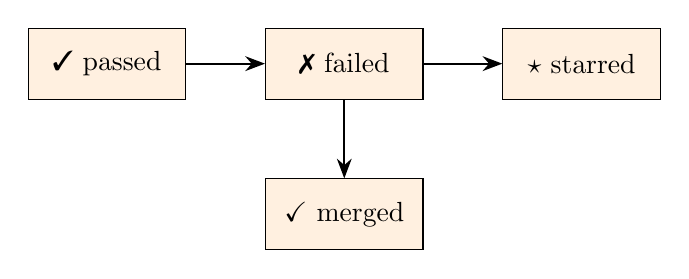
\begin{tikzpicture}[node distance=1cm]
    \node[sq] (a) {\ding{51}\ passed};
    \node[sq, right=of a] (b) {\ding{55}\ failed};
    \node[sq, right=of b] (c) {$\star$ starred};
    \node[sq, below=of b] (d) {$\checkmark$ merged};
    \draw[arr] (a) -- (b);
    \draw[arr] (b) -- (c);
    \draw[arr] (b) -- (d);
  \end{tikzpicture}
\end{frame}

\begin{frame}{Big math in boxes}
  \centering
  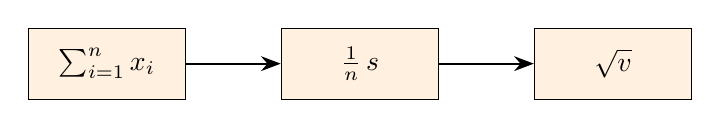
\begin{tikzpicture}[node distance=1.2cm]
    \node[sq] (a) {$\sum_{i=1}^{n} x_i$};
    \node[sq, right=of a] (b) {$\frac{1}{n}\,s$};
    \node[sq, right=of b] (c) {$\sqrt{v}$};
    \draw[arr] (a) -- (b);
    \draw[arr] (b) -- (c);
  \end{tikzpicture}
\end{frame}

\begin{frame}{Numbered step circles on arrows}
  \centering
  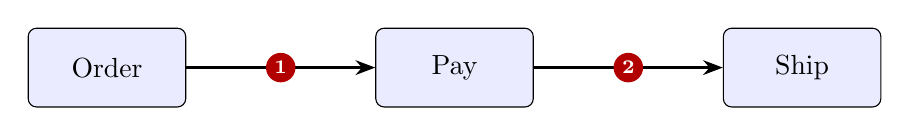
\begin{tikzpicture}[node distance=2.4cm,
      num/.style={circle, fill=red!70!black, text=white, font=\scriptsize\bfseries, inner sep=1.5pt}]
    \node[box] (a) {Order};
    \node[box, right=of a] (b) {Pay};
    \node[box, right=of b] (c) {Ship};
    \draw[arr] (a) -- node[num] {1} (b);
    \draw[arr] (b) -- node[num] {2} (c);
  \end{tikzpicture}
\end{frame}

% --- Annotated arrows -------------------------------------------------------------------------

\begin{frame}{Two-line labels on arrows}
  \centering
  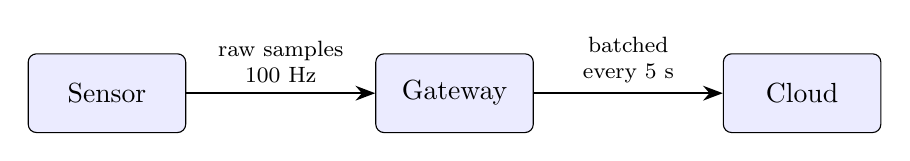
\begin{tikzpicture}[node distance=2.4cm]
    \node[box] (a) {Sensor};
    \node[box, right=of a] (b) {Gateway};
    \node[box, right=of b] (c) {Cloud};
    \draw[arr] (a) -- node[above, note, align=center] {raw samples\\100 Hz} (b);
    \draw[arr] (b) -- node[above, note, align=center] {batched\\every 5 s} (c);
  \end{tikzpicture}
\end{frame}

\begin{frame}{Labels sitting on the line}
  \centering
  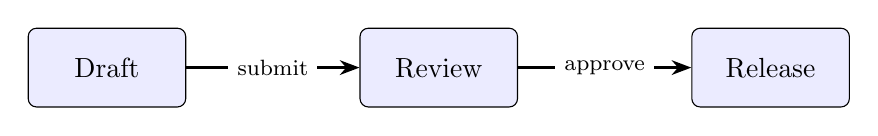
\begin{tikzpicture}[node distance=2.2cm]
    \node[box] (a) {Draft};
    \node[box, right=of a] (b) {Review};
    \node[box, right=of b] (c) {Release};
    \draw[arr] (a) -- node[fill=white, note] {submit} (b);
    \draw[arr] (b) -- node[fill=white, note] {approve} (c);
  \end{tikzpicture}
\end{frame}

\begin{frame}{Request and response arrows}
  \centering
  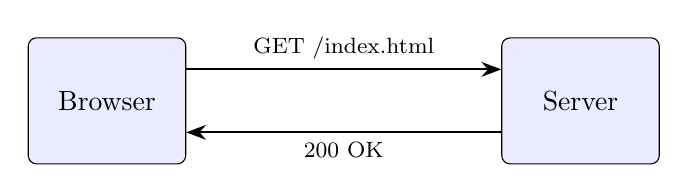
\begin{tikzpicture}[node distance=4cm]
    \node[box, minimum height=1.6cm] (a) {Browser};
    \node[box, minimum height=1.6cm, right=of a] (b) {Server};
    \draw[arr] ([yshift=4mm]a.east) -- node[above, note] {GET /index.html} ([yshift=4mm]b.west);
    \draw[arr] ([yshift=-4mm]b.west) -- node[below, note] {200 OK} ([yshift=-4mm]a.east);
  \end{tikzpicture}
\end{frame}

\begin{frame}{Math on arrows}
  \centering
  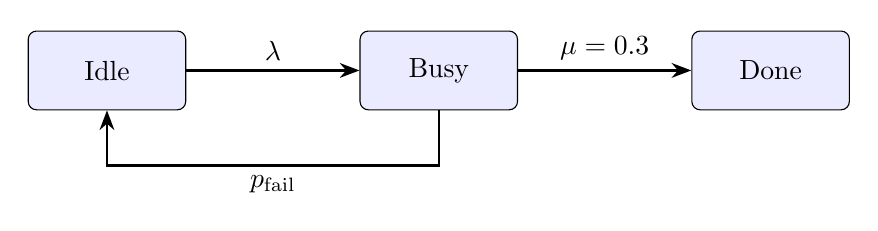
\begin{tikzpicture}[node distance=2.2cm]
    \node[box] (a) {Idle};
    \node[box, right=of a] (b) {Busy};
    \node[box, right=of b] (c) {Done};
    \draw[arr] (a) -- node[above] {$\lambda$} (b);
    \draw[arr] (b) -- node[above] {$\mu = 0.3$} (c);
    \draw[arr] (b.south) -- ++(0,-0.7) -| node[pos=0.25, below] {$p_{\mathrm{fail}}$} (a.south);
  \end{tikzpicture}
\end{frame}

\begin{frame}{Coloured and italic labels on dashed arrows}
  \centering
  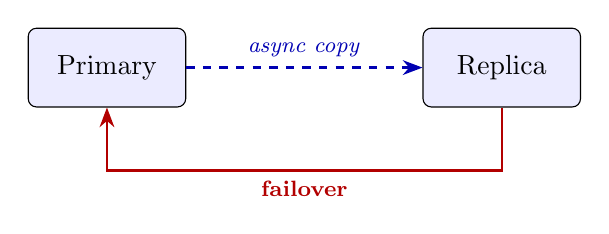
\begin{tikzpicture}[node distance=3cm]
    \node[box] (a) {Primary};
    \node[box, right=of a] (b) {Replica};
    \draw[arr, dashed, blue!70!black] (a) -- node[above, note, text=blue!70!black] {\emph{async copy}} (b);
    \draw[arr, red!70!black] (b.south) -- ++(0,-0.8) -| node[pos=0.25, below, note, text=red!70!black]
      {\textbf{failover}} (a.south);
  \end{tikzpicture}
\end{frame}

\begin{frame}{Labels beside vertical arrows}
  \centering
  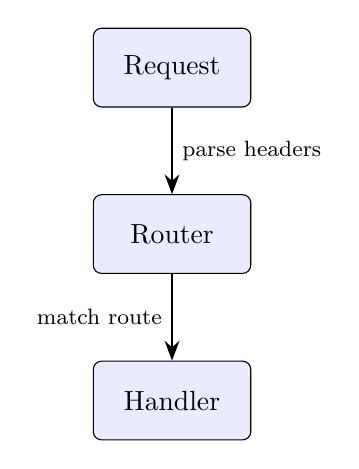
\begin{tikzpicture}[node distance=1.1cm]
    \node[box] (a) {Request};
    \node[box, below=of a] (b) {Router};
    \node[box, below=of b] (c) {Handler};
    \draw[arr] (a) -- node[right, note] {parse headers} (b);
    \draw[arr] (b) -- node[left, note] {match route} (c);
  \end{tikzpicture}
\end{frame}

\begin{frame}{An icon and words on one arrow label}
  \centering
  \begin{tikzpicture}[node distance=3.4cm]
    \node[box] (a) {Phone};
    \node[box, right=of a] (b) {Bank};
    \draw[arr] (a) -- node[above, note] {\faLock\ TLS 1.3} (b);
    \draw[arr] (b) -- ++(0,-1.2) -| node[pos=0.25, below, note] {\faCheck\ confirmed} (a);
  \end{tikzpicture}
\end{frame}

% --- Whole schematics -------------------------------------------------------------------------

\begin{frame}{A cloud architecture with logos}
  \centering
  \begin{tikzpicture}[node distance=0.6cm and 1cm, mini/.style={card, minimum height=1.6cm, minimum width=1.8cm}]
    \node[mini] (u) {\icon[0.6cm]{icon_user.png}\\ \footnotesize Users};
    \node[mini, right=of u] (lb) {\icon[0.6cm]{icon_cloud.png}\\ \footnotesize Load balancer};
    \node[mini, right=of lb, yshift=1.1cm] (s1) {\icon[0.6cm]{icon_gear.png}\\ \footnotesize App 1};
    \node[mini, right=of lb, yshift=-1.1cm] (s2) {\icon[0.6cm]{icon_gear.png}\\ \footnotesize App 2};
    \node[mini, right=of s1, yshift=-1.1cm] (db) {\icon[0.6cm]{icon_db.png}\\ \footnotesize Database};
    \begin{scope}[on background layer]
      \node[draw, dashed, rounded corners, fit=(s1)(s2), inner sep=6pt, label={[note]above:region A}] {};
    \end{scope}
    \draw[arr] (u) -- node[above, note] {HTTPS} (lb);
    \draw[arr] (lb) -- (s1);
    \draw[arr] (lb) -- (s2);
    \draw[arr] (s1) -- (db);
    \draw[arr] (s2) -- (db);
  \end{tikzpicture}
\end{frame}

\begin{frame}{A data pipeline with icons and step numbers}
  \centering
  \begin{tikzpicture}[node distance=1.5cm,
      num/.style={circle, fill=blue!60!black, text=white, font=\scriptsize\bfseries, inner sep=1.5pt}]
    \node[card] (a) {{\Large\faFileCsv}\\ Extract};
    \node[card, right=of a] (b) {{\Large\faFilter}\\ Transform};
    \node[card, right=of b] (c) {\icon[0.6cm]{icon_db.png}\\ Load};
    \node[num] at (a.north west) {1};
    \node[num] at (b.north west) {2};
    \node[num] at (c.north west) {3};
    \draw[arr] (a) -- node[above, note] {rows} (b);
    \draw[arr] (b) -- node[above, note] {clean rows} (c);
  \end{tikzpicture}
\end{frame}

\begin{frame}{Swimlanes with logo headers}
  \centering
  \begin{tikzpicture}[lane/.style={draw, fill=gray!8, minimum width=3.2cm, minimum height=4.2cm},
      task/.style={sq, minimum width=2.4cm, minimum height=0.7cm, font=\footnotesize}]
    \node[lane] (l1) at (0,0) {};
    \node[lane] (l2) at (3.4,0) {};
    \node[anchor=north] at (l1.north) {\icon[0.5cm]{icon_user.png}\ \small Customer};
    \node[anchor=north] at (l2.north) {\icon[0.5cm]{icon_gear.png}\ \small Shop};
    \node[task] (t1) at (0,0.6) {Place order};
    \node[task] (t2) at (3.4,0.6) {Check stock};
    \node[task] (t3) at (3.4,-0.6) {Ship};
    \node[task] (t4) at (0,-1.5) {Receive};
    \draw[arr] (t1) -- (t2);
    \draw[arr] (t2) -- (t3);
    \draw[arr] (t3) |- (t4);
  \end{tikzpicture}
\end{frame}

\begin{frame}{A system context diagram}
  \centering
  \begin{tikzpicture}[node distance=1cm and 1.6cm,
      ext/.style={draw, dashed, rounded corners=3pt, fill=gray!10, minimum height=1cm, minimum width=2.4cm, align=center}]
    \node[align=center] (p) {\icon[1cm]{icon_user.png}\\ \small Customer};
    \node[box, fill=blue!25, minimum width=3cm, minimum height=1.4cm, right=of p] (s) {\textbf{Booking system}\\ \footnotesize books rooms};
    \node[ext, above right=of s] (pay) {Payments\\ \footnotesize external};
    \node[ext, below right=of s] (mail) {Email\\ \footnotesize external};
    \draw[arr] (p) -- node[above, note] {books} (s);
    \draw[arr] (s) -- node[above left, note] {charges} (pay);
    \draw[arr] (s) -- node[below left, note] {notifies} (mail);
  \end{tikzpicture}
\end{frame}

\begin{frame}{A smartdiagram flow}
  \centering
  \smartdiagram[flow diagram:horizontal]{Plan, Build, Test, Ship}
\end{frame}

\end{document}
